\documentclass[letterpaper, 11pt, twocolumn]{article}
\usepackage[margin=1in]{geometry}
\setlength{\columnsep}{0.75cm}

\usepackage{tikz}
\usetikzlibrary{calc}
\usepackage{algorithm2e}
\usepackage{multirow}
\usepackage{graphicx}
\usepackage{amsmath}
\usepackage{cite}
\usepackage{framed, color}
\usepackage{color, soul}
\definecolor{shadecolor}{rgb}{.93,.93,.93}
\definecolor{blu}{rgb}{0,0,1}
\newcommand{\td}[1]{{\color{blu}\hl{TODO: #1}}}
\newcommand{\vwm}{$V_{w,n,k}$}
\newcommand{\wm}{$W_{w,n,k}$}
\usepackage{amssymb}
\usepackage{mathrsfs}
\usepackage{gensymb}

\title{Climate control for performant HPUs}
\author{}
 
\parindent0pt \parskip8pt
\begin{document}
\maketitle

\section*{Abstract}
\textbf{}
\section*{Introduction}
There are still many tasks for which humans outperform computers
These tend to be tasks that rely on a large repertoire of prior knowledge,
the excercise of common sense judgment, certain visual tasks, and 
tasks that require spontaneous hypothesis generation.

With the emergence of microtask platforms like Amazon Mechanical Turk (AMT),
comes the hope of building compute in which human intelligence can be accessed
on-demand.  This leads to an analogy of the human to the CPU, wherein we think
of human processing units.

A major challenge in building systems that deliver on this vision is the 
natual variability obtained in HPU output.  In some tasks, this variability
is desireable.  For example, in an image labelling task, the natural 
variability in
HPU output leads to greater coverage of the semantic space occupied by an 
image.  In other cases this variability can be problematic, such as in a 
transcription task, where there is only one corect output, and any variability
is only noise.

Whether desired or not, to build up efficient systems from HPUs, one must 
understand the natural variance quantitatively, and understand the factors that
influence it.

Here we model the variance between HPUs as comming from two sources.  The first
is a persistent, or intrinsic variability.  We imagine that this to encompass  
temperamental predispositions, life history, and developmental stage of the 
individual.  While
it may change over the course of a person's lifetime, in the view of the 
computational architect, it is essentially constant.

The seccond is a short-term variability, which arises from the fact that 
peoples immediate state is a function of recent events.  This would include
such things as an HPU becomming more efficient at a task once it has completed
a few tasks of the same type.  It would also include such things as the 
potentially detrimental effects of a noisy environment.

In this view, one can imagine HPUs being different in their specifications,
and also exhibiting hysteresis, whereby their output at some time $t$ is a
function of their inputs at time $t$, $t-1$, and so on.

In psychology, the act of producing these short-lived states that effect a
person's performance during a task is called \textit{priming}.  We will adopt
this term throughout the present work.


\section*{Prior Work}
Priming itself can be broken into many types, and many studies exist exploring
the effects of overt priming on the performance of HPUs. Priming may arise
due to how the task is framed.  This includes such things as the stated
purpose of the task, and the identity of the requester the task.

In \cite{chandler2013breaking}, the researchers investigate the effects of 
framing task either in a meaningful or meaningless way.  Compared to a 
zero-context control treatment, workers increase their output (for less pay),
when they are told that they are helping identify cancer, but there is no
change in quality.  When workers are told that their submissions will be 
discarded, there is no change in the amount of work done, but the quality 
declines.

Another source of priming can be due to what might be called 
\textit{sidestream information}: information that is presented to the 
individual but which is not actually salient to the task.

Other researchers have studied how having peer's responses available to 
the task could influence the worker.

In the present work, we focus on a more subtle source of priming, which arises
simply from the worker's performance in earlier stages of the task. 

We compare this to priming arising from framing the task by disclosing a 
(fictitious) funding agency that is paying for the study in which they are 
participating.

\section*{Methods}

We paid 900 AMT workers to perform an image-labelling task.  Each worker
was randomly assigned to one of 6 priming treatments. A task consisted of 
labelling 10 images, with 5 labels each.  The first 5 images were varied 
depending on the priming treatment, and this was used to explore the effects
of \textit{in-task} priming.  The last 5 images were the same accross all 
treatments, and served as the primary means of assessing the effects of 
the priming treatments.

The test images were chosen with two ideals in mind.  First, we chose images
that we felt would generate a diverse vocabulary of labels, such that the
effects of priming could be detected.  Images that are sparse, and with a 
very strong foreground might produce a narrow distribution of labels that 
would not exhibit the effects of priming as much.  

Second, we chose images which would produce labels belonging to two broad
concepts, food and culture.  The purpose of this was to test to what
extent workers could be biased in favor of focusing on one concept or the other
during labelling.

We divide our treatments into three broad classes: \textit{ambiguous}, 
\textit{culture}, and \textit{food}.
\section*{Results}
\begin{figure*}
	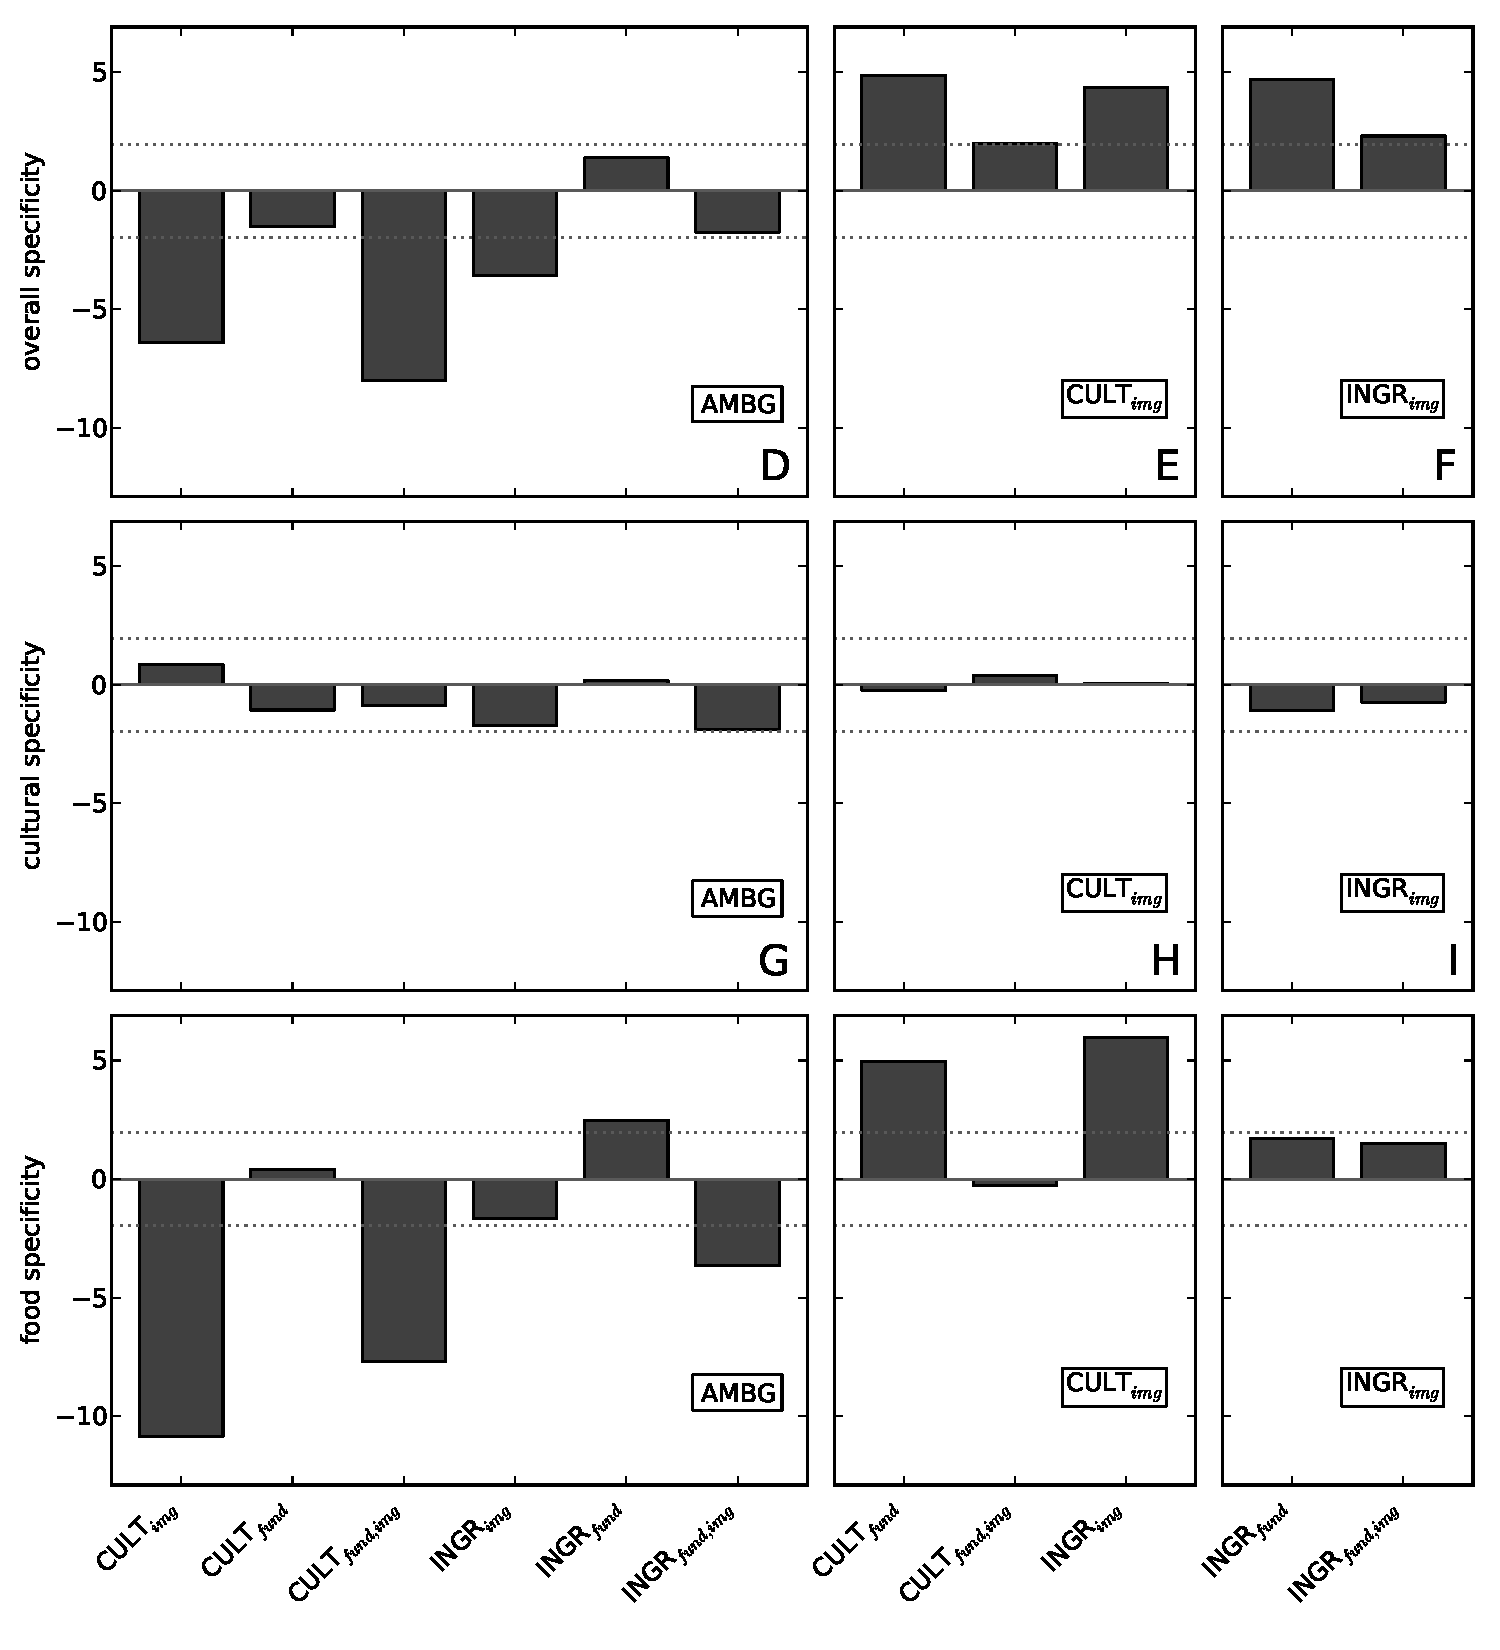
\includegraphics[scale=0.65]{../figs/specificity.pdf}
\end{figure*}

\bibliographystyle{plain}
\bibliography{bab.bib}
\end{document}
